\documentclass[notitlepage]{report}
\usepackage[left=1in, right=1in, top=1in, bottom=1in]{geometry}

\usepackage{titling}
\usepackage{graphicx}
\usepackage{fullpage}

\pretitle{\begin{center}\Huge\bfseries}
\posttitle{\par\end{center}\vskip 0.5em}
\preauthor{\begin{center}\Large\ttfamily}
\postauthor{\end{center}}
\predate{\par\large\centering}
\postdate{\par}

\title{A Brief Dive into Graph Isomorphism}
\author{Kevin Richard Koch}
\date{\today}
\begin{document}

\maketitle
\thispagestyle{empty}

\begin{abstract}
In this paper I will explain my exploration of graph isomorphism as a problem in computer science, as well as an algorithm I discovered written by Ullmann in 1976. The algorithm explores a subset of the graph isomorphism problem, sub graph isomorphism. I will also go into some of the real world applications of Graph Isomorphism, as well as the history and future for the topic.
\end{abstract}

\section*{What is graph isomorphism}
Graph Isomorphism, here after refereed to as GI, is a characteristic of a graph to be able to be rewritten in different ways, while still maintaining the same information.
\begin{figure}[h!]
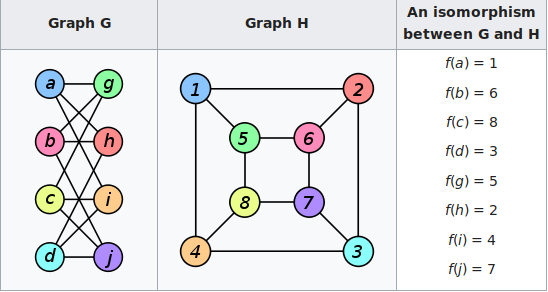
\includegraphics[width=\linewidth]{/home/cptwalmart/Documents/COSC320/Graph-Isomorphism-Project/images/WikiGraphIsomorphismExample.png}
\caption{An example of an isomorphic graph}
\end{figure}

As you can see from the two graphs, even though they look very dissimilar, they are infarct the same graph. This property is extremely useful in many fields today. Chemists are able to look at the molecular makeup of different substances, and use GI to identify known atomic structures. This aspect of GI is so researched in fact that it is known as the "Chemist's Problem".

I should also take a moment to address what exactly is the Graph Isomorphism problem. Suppose that $\omega^{1}$ and $\omega^{2}$ are two graphs with $n$ vertices, the GI problem asks if they are isomorphic or not. GI plays an important role in Computer Theory because it lies in the class known as NP, and is rated NP-Hard. It is unknown if it lies in P or NP-Complete, however most heuristic evidience stronly implies that it is not NP-Complete. Further evidence of this is the fact that if it was proven that this is NP-Complete, then the polynomial hierarchy would collapse. GI is known to be polynomial complete for graphs of bounded degree, bounded genus, bounded eigenvalue mutiplicity, and treewidth. The problem of counting the number of isomorphisms between two graphs is Turing reducible to the inversion of the graph itself. It is known that it has a time complexity of at most exp$(O(n^{2/3}))$ for a graph with V(n). Also there are plenty of general algorithms for GI wheich are "practical in practice" meaning there are some worst case inputs which cause it to have a horrendius run time, however for most it is fine.  ~\cite{derksen, hartke}


Now before we continue, I should define some terminology so it is known when referenced later on in the paper. A graph through this paper shall be known as an \textit{combinatorial graph}. So, a graph G is a finite set of \textit{vertices} plus a set of ordered or unordered pairs of vertices named \textit{edges}. A set of vertices shall be noted as \textit{V(G)} while a set of edges will be noted as \textit{E(G)}. Graphs containing ordered pairs shall be known as \textit{directed} and ones with unordered pairs shall be known as \textit{undirected}. Graphs shall be assumed to be undirected unless otherwise noted. The number of edges of a vertex shall be known as a \textit{valence} of the vertex. For a vertex, the number of head ends adjacent to a vertex is called the \textit{indegree} of the vertex and the number of tail ends adjacent to a vertex is its \textit{outdegree}. (How many nodes point to it, and how many point out)A \textit{connected component} is a subgraph in which any two vertices are connected to each other by paths, and which is connected to no additional vertices in the supergraph. A \textit{loop} is an edge that connects a vertex to itself. And finally a \textit{parallel edge} are two or more edges which are incident to the same two vertices.

\subsection*{Properties of Graph Isomorphism}
For a graph to be isomorphic, it must fulfill several criteria. Not every graph that looks similar are isomorphic, one key feature of an isomorphic graph is that $V^{1}(G) = V^{2}(G)$, and $E^{1}(G) = E^{1}(G)$. There must exist a one to one mapping between the graph's vertices, and the following properties are satisfied, then the two graphs are said to be isomorphic.

\begin{enumerate}
\item $V^{1}(G) = V^{2}(G)$
\item $E^{1}(G) = E^{1}(G)$
\item The indegree and outdegree should be equal
\item The number of connected components should be the same
\item The number of loops should be the same
\item The number of parallel edges should be the same
\end{enumerate}

\section*{The Chemist's problem}
This problem is actually identifying what molecule is what. Say you're given the molecule for water, which is commonly known as H$_{2}$O. You would have to analyze different structures and try and match it with water. So efficient graph isomorphism algorithms are super convenient here, since molecules can be made into a graph form where the bonds would be the edges, and the vertexes would be the different atoms that make up the compound.~\cite{miller}





\bibliography{bib}
\bibliographystyle{plain}


\end{document}